\section{Notre Contribution : Tétraèdres en Diamants}
\subsection{Principe général}
\noindent
Notre algorithme s'inspire fortement de SQUAD. Seulement, appareiller les tétraèdres deux à deux permet seulement d'économiser une référence par cube, c'est à dire de passer de 4 références par tétraèdre à 3.\\
L'idée ici est de regrouper les tétraèdres partageant une même arête. On appelle un tel regroupement : \textbf{un diamant}. Notre algorithme plusieurs idées :
\begin{itemize}
\item Regroupement des tétraèdres comme SQUAD
\item Ancrer un sommet avec un diamant comme SOT
\item Ordonner les diamants tel-que le ième sommet soit au sein du ième diamant comme SOT
\item Passage d'un tétraèdre à l'autre en utilisant les faces (et non les coins)\\
\end{itemize}
Un diamant est un ensemble de tétraèdres adjacents deux à deux, partageant une arête commune et formant un cycle (Fig. \ref{fig:full_diamond2}). Dès lors que l'ensemble des tétraèdres n'est pas cyclique, la figure géométrique n'est plus un diamant (Fig. \ref{fig:not_full_diamond}).
\begin{figure}[H]
\centering
\begin{subfigure}{.5\textwidth}
  \centering
  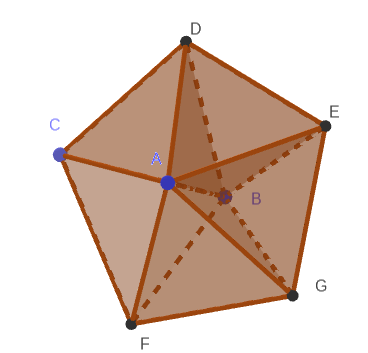
\includegraphics[scale=0.3]{Images/full_diamond}
  \caption{}
  \label{fig:full_diamond2}
\end{subfigure}%
\begin{subfigure}{.5\textwidth}
  \centering
  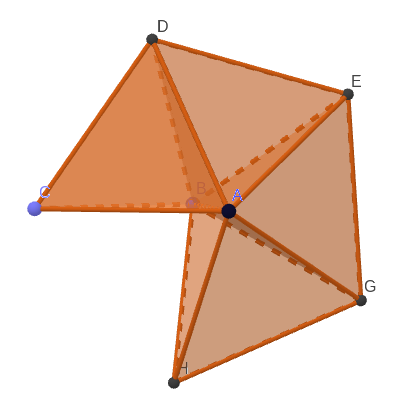
\includegraphics[scale=0.26]{Images/not_full_diamond}
  \caption{}
  \label{fig:not_full_diamond}
\end{subfigure}
\caption{\textbf{Gauche} : Exemple de diamant contenant 5 tétraèdres et dont l'arête centrale commune est AB. \textbf{Droite} : Exemple n'étant pas un diamant car les tétraèdres ne sont pas cycliques (bien que tous les tétraèdres partagent la même arête AB)}
%\label{fig:kvqkq}
\end{figure}
\noindent
Au sein d'un diamant, les tétraèdres sont ordonnés. Ainsi, on peut oublier les références de voisinage entre deux tétraèdres du même diamant. Pour les tétraèdres au sein d'un diamant, seules les références vers des tétraèdres extérieurs au diamant sont nécessaires. Un diamant $D_i$ contenant $|D_i|$ tétraèdres a $2|D_i|$ faces extérieures donc $2|D_i|$ références. Sur la Fig. \ref{fig:full_diamond2}, les faces ABD,ABE,ABG,ABF,ABC n'apparaitront pas dans notre structure car nous savons implicitement que pour passer d'un tétraèdre à l'autre dans ce diamant, nous utilisons une de ces faces.

\subsection{Appariement des tétraèdres en diamants}
\noindent
La première étape consiste à regrouper les tétraèdres en diamants. On peut ramener ce problème à un problème d'optimisation dans les graphes. En considérant notre maillage tétraèdrique comme un graphe (i.e en ne conservant que les arêtes et les sommets), il s'agit de choisir un ensemble $E'$ d'arêtes tel-que deux arêtes de $E'$ n'appartiennent pas au même tétraèdre. Les arêtes candidates pour appartenir à $E'$ sont toutes les arêtes qui ne sont pas situées sur les bords du maillage. Par exemple, sur Fig. \ref{fig:not_full_diamond}, l'arête AB est située sur le bord du maillage et n'est donc pas candidate pour appartenir à $E'$. Pour chaque arête selectionnée, le diamant est constitué de tous les tétraèdres possédant cette arête. Tous les tétraèdres n'ayant pas d'arêtes dans $E'$ sont appelés les tétraèdres isolés.\\
Pour trouver cet ensemble d'arêtes, nous avons essayé plusieurs algorithmes.
\subsubsection{Choisir une direction pour chaque sommet}
\noindent
La première méthode consiste à prendre pour chaque sommet, une arête dans une direction pré-définie. Néanmoins, cette méthode a deux inconvénients majeurs : deux arêtes peuvent être choisies et appartenir au même tétraèdre et elle utilise la géometrie du domaine (et donc peut sembler moins générique). Nous avons donc choisi de ne pas utiliser cette méthode.

\subsubsection{Optimisation aléatoire}
\noindent
Notre problème s'exprime facilement comme un problème d'optimisation combinatoire en nombres entiers. Malheureusement, la résolution de ces problèmes est NP-difficile, ce qui signifie qu'aucun algorithme ne peut trouver une solution optimale en temps polynomial. Néanmoins, on peut utiliser des algorithmes d'optimisation aléatoire afin de trouver une solution approchée. Ce sont des algorithmes très utilisés en pratique qui visitent plus ou moins aléatoirement l'espace des solutions.\\
Soit $f$ la fonction aléatoire à maximiser, l'idée est de partir d'une solution initiale x et tant que la condition d'arrêt n'est pas remplie, de créer une solution y à partir de x puis de remplacer x par y si f(y)$>$f(x).\\
Dans notre cas, une solution est un ensemble d'arêtes. Elle est faisable si pour toute paire d'arêtes de notre solution, aucunes n'appartiennent au même tétraèdre. On peut donc matérialiser notre solution comme un vecteur de 0 et 1 pour chaque arête du graphe (1 si l'arête appartient à la solution, 0 sinon). Pour calculer la valeur de notre solution, on ajoute pour chaque arête de la solution le nombre de tétraèdres utilisant l'arête et si deux arêtes appartiennent au même tétraèdre alors on inflige une pénalité en soustrayant le nombre de tétraèdres adjacents à ces deux arêtes. L'inconvénient majeur de cet algorithme est sa lenteur. Il permet de trouver des solutions quasi optimales pour des maillages avec quelques milliers d'arêtes rapidement mais ne permet pas de trouver des solutions convenables au dela dans un temps raisonable. Nous avons donc décidé de ne pas retenir cette solution.

\subsubsection{Choisir l'arête de degré maximum}
\noindent
Le degré d'une arête est le nombre de tétraèdres possédant cette arête. Une heuristique très simple consiste à prendre en priorité les arêtes ayant un degré important. C'est un algorithme glouton dans la mesure où seulement la récompense immédiate nous intéresse. Il est nécessaire de trouver l'arête maximum à chaque itération de l'algorithme et cela a pour conséquence un temps d'exécution relativement long.
\subsubsection{Parcours en largeur des tétraèdres}
\label{parcours_largeur}
\noindent
La troisième approche consiste à parcourir le maillage en largeur. On choisit un tétraèdre au début de l'algorithme puis on regarde pour chacune de ses arêtes si les tétraèdres partageant cette arête forment un diamant et qu'aucun n'appartienne déja à un diamant. Si ces deux conditions sont remplies, on crée un nouveau diamant avec cette arête centrale. Puis on ajoute à la file les tétraèdres adjacents et non visités au tétraèdre choisi. On exécute ainsi cet algorithme tant que la file n'est pas vide.\\
\begin{algorithm}[th]
\SetAlgoLined	
 Soit F une file;\\
 F.ajouter(t);\\
 \While{F n'est pas vide}{
  t = F.défiler();\\
  \For{arête e dans t}{
  \If{e forme un diamant}{
  \If{aucun des tétraèdres ayant e n'appartient à un diamant}{
  Creer un diamant avec e comme arête centrale;\\
  }
  }
  }
  Marquer t;\\
  Ajouter voisins de t non marqués à Q;
 }
 \caption{Parcours en largeur du maillage avec un tétraèdre de départ t}
\end{algorithm}

\begin{figure}[H]
\centering
\begin{subfigure}{.5\textwidth}
  \centering
  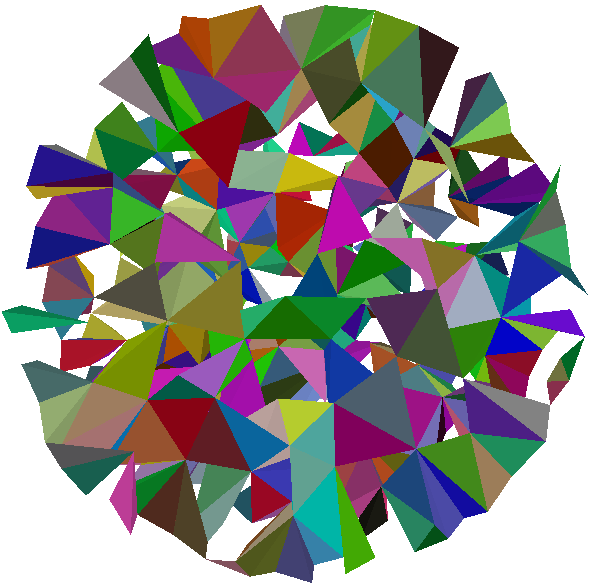
\includegraphics[scale=0.2]{Images/isolated_tetra}
  \caption{}
  \label{fig:isolated_tetra}
\end{subfigure}%
\begin{subfigure}{.5\textwidth}
  \centering
  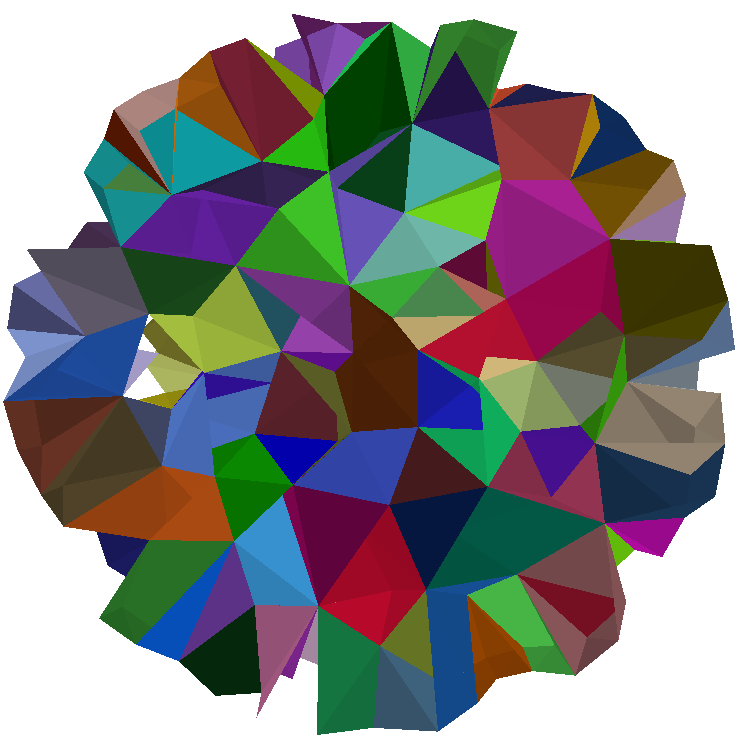
\includegraphics[scale=0.16]{Images/diamond}
   \caption{}
  \label{fig:diamond}
\end{subfigure}
\caption{\textbf{Gauche} : Vue de coupe des tétraèdres isolés après exécution du parcours en largeur pour créer les diamants. Chaque couleur représente un tétraèdre isolé. \textbf{Droite} : Vue de coupe des diamants après exécution du parcours en largeur pour créer les diamants. Chaque couleur représente un diamant.}
\end{figure}
\noindent
Sur Fig. \ref{fig:isolated_tetra}, on note une certaine homogénéité des tétraèdres isolés. En analysant plus spécifiquement la concentration des tétraèdres isolés, on remarque sur la Fig. \ref{fig:density_cow_hand} qu'ils sont particulièrement situé sur les bords et dans des régions à courbures \footnote{Afin que la densité ne soit pas biaisée, nous avons soustrait la densité originale du maillage. Le fait qu'une région soit plus densément peuplée en tétraèdres n'influence donc pas le résultat.}.
\begin{figure}[H]
\centering
\begin{subfigure}{.5\textwidth}
  \centering
  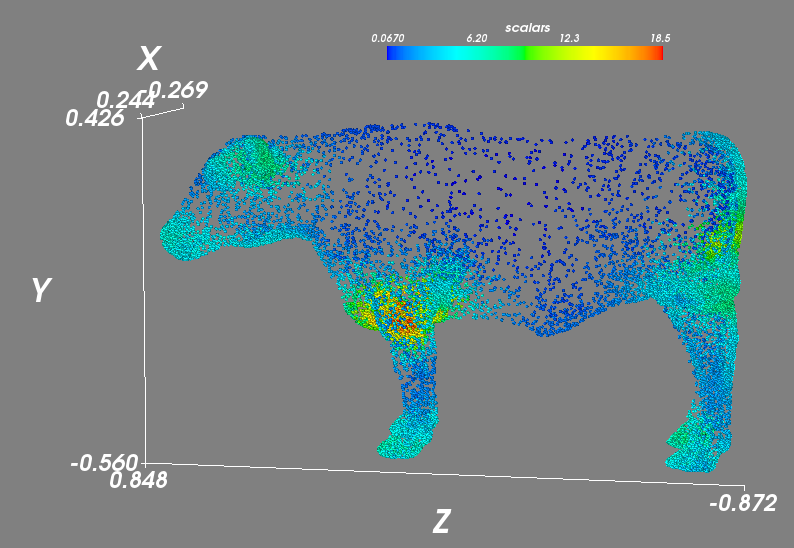
\includegraphics[scale=0.25]{Images/density_cow}
\end{subfigure}%
\begin{subfigure}{.5\textwidth}
  \centering
  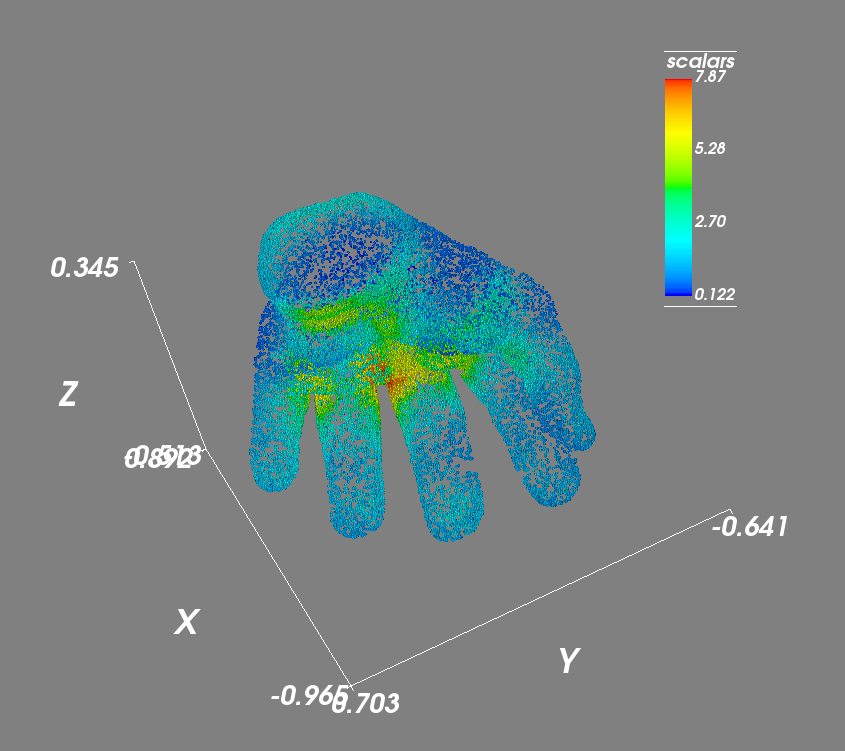
\includegraphics[scale=0.22]{Images/hand_density}
\end{subfigure}
\caption{Distribution des tétraèdres isolés. Chaque point représente le barycentre d'un tétraèdre et sa couleur indique la densité (le nombre de tétraèdres isolés à proximité).}
\label{fig:density_cow_hand}
\end{figure}

\paragraph{Choix du tétraèdre de départ}
Suivant le premier tétraèdre choisi pour lancer l'algorithme de parcours en largeur (Fig. \ref{fig:bfs_starting}), le taux de tétraèdres appareillés dans des diamants varie peu (1\% d'écart). Il semble néanmoins plus intéressant de commencer par les régions étroites.
\begin{figure}[H]
\begin{center}
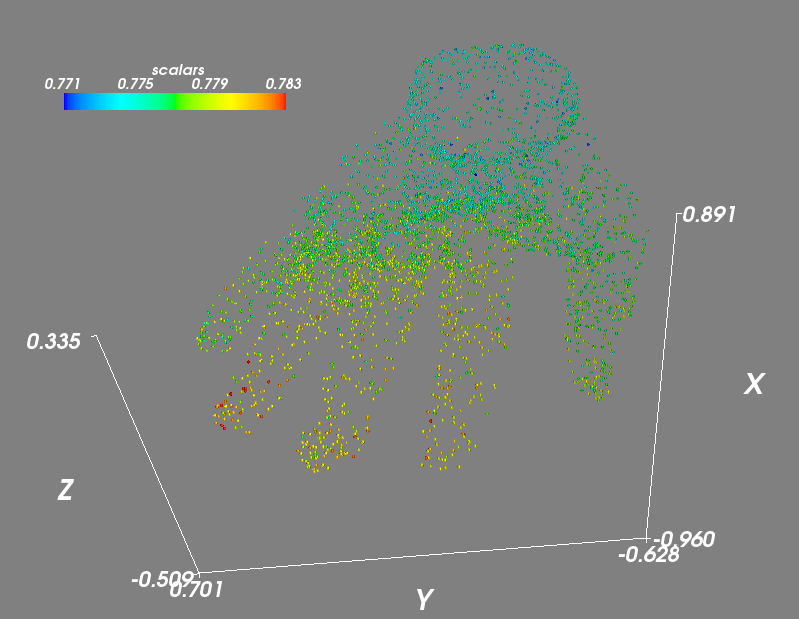
\includegraphics[scale=0.22]{Images/bfs_starting}
\caption{Performance de l'algorithme de parcours en largeur en fonction du tétraèdre de départ.}
\label{fig:bfs_starting}
\end{center}
\end{figure}

%\subsubsection{Résultats}


%\begin{tikzpicture}
%\begin{axis}[
%    title={Evolution des rpt en fonction du nombre de tétraèdres},
%    xlabel={Nombre de tétraèdres},
%    ylabel={RPT},
%    xmin=3000, xmax=2500000,
%    ymin=2, ymax=3,
%    xmode=log,
%%    xtick={0,20,40,60,80,100},
%%    ytick={0,20,40,60,80,100,120},
%    legend pos=north west,
%    ymajorgrids=true,
%    grid style=dashed,
%]
% 
%\addplot[
%    color=blue,
%    mark=square,
%    ]
%    coordinates {
%    (3583,2.69)(83412,2.39)(125127,2.44)(134707,2.44)(144037,2.37)(156135,2.44)(2243131,2.37)
%    };
%%    \legend{CuSO$_4\cdot$5H$_2$O}
% 
%\end{axis}
%\end{tikzpicture}

\subsection{Choisir l'ancre}
\label{ancrage}
\noindent
\begin{figure}[H]
\begin{center}
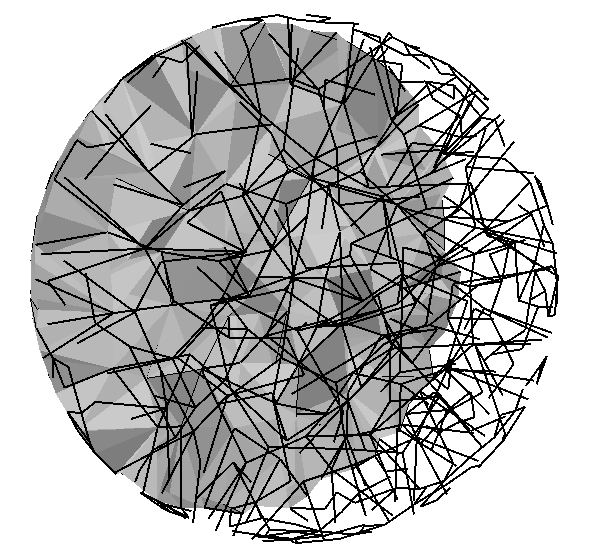
\includegraphics[scale=0.2]{Images/central_edges}
\caption{Vue de coupe d'une tétraèdrisation d'une boule avec affichage des arêtes centrales de tous les diamants}
\label{fig:central_edges}
\end{center}
\end{figure}
\noindent
Le but de cette section est d'associer chaque sommet à un diamant ou un tétraèdre isolé. Voici les règles pour l'association.\\
\begin{itemize}
\item Un diamant ne peut être associé qu'à un sommet de son arête centrale
\item Un tétraèdre isolé peut être associé à n'importe lequel de ses quatres sommets
\item On associe en priorité les sommets à des diamants afin de calculer plus rapidement le degré du sommet\\
\end{itemize}
Les différents cas possibles pour l'association des sommets sont les suivants :\\
\begin{itemize}
\item Le sommet est adjacent à une arête centrale disponible. On associe le sommet à cette arête.
\item Le sommet n'est adjacent à aucune arête centrale et il est adjacent à un tétraèdre isolé libre. Alors on associe le sommet à ce tétraèdre libre.
\item Le sommet n'est adjacent à aucune arête centrale, n'est pas adjacent à un tétraèdre isolé libre mais est adjacent à un diamant. On 'explose' alors le diamant, c'est à dire qu'on fait comme s'il était constitué que de tétraèdres isolés. Sur la Fig. \ref{fig:central_edge_AB}, le sommet F n'est pas sur une arête centrale. Si le diamant est déjà associé au sommet A (resp. B) alors on explose le diamant. On peut alors associer le sommet F (Fig. \ref{fig:explosion_diamond}) aux tétraèdres ABFG ou ABFC et le sommet A (resp. B) aux tétraèdres ACDB ou ADEB ou ABEG.\\
\end{itemize}

\begin{figure}[H]
\centering
\begin{subfigure}{.5\textwidth}
  \centering
  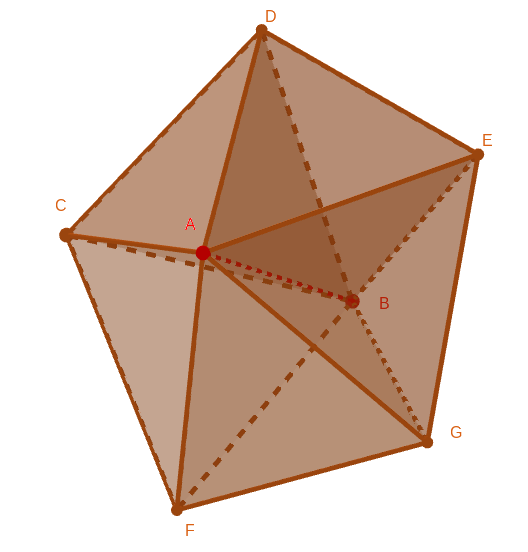
\includegraphics[scale=0.25]{Images/central_edge_AB}
  \caption{}
  \label{fig:central_edge_AB}
\end{subfigure}%
\begin{subfigure}{.5\textwidth}
  \centering
  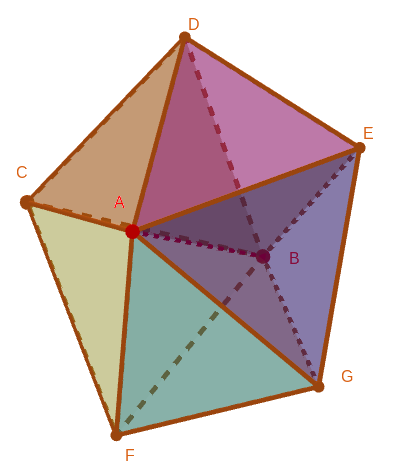
\includegraphics[scale=0.32]{Images/explosion_diamond}
  \caption{}
  \label{fig:explosion_diamond}
\end{subfigure}
\caption{\textbf{Gauche} : Diamant contenant 5 tétraèdres dont l'arête centrale est le segment AB et ancré au sommet A. \textbf{Droite} : 5 tétraèdres isolés (chaque couleur est un tétraèdre différent)}
\end{figure}
\noindent
Afin d'ancrer les sommets aux diamants/tétraèdres isolés, nous appliquons un algorithme glouton affectant en priorité les sommets adjacents à peu d'arêtes centrales et de tétraèdres isolés. Puis si nécessaire, nous explosons des diamants afin que tous les sommets soient appareillés avec des diamants/tétraèdres isolés différents.

\subsection{Organisation des diamant, tétraèdres et sommets}
\noindent
Les diamants sont construits et les sommets sont appareillés avec des diamants ou des tétraèdres isolés. Nous allons désormais apporter des précisions sur la manière dont sont ordonnés les diamants, tétraèdres et sommets.
\paragraph{Ordre des tétraèdres dans un diamant}
Au sein d'un diamant les tétraèdres sont ordonnés de manière purement arbitraire (Fig. \ref{fig:tetra_ordonnee}). La seule condition est que deux tétraèdres adjacents doivent avoir un ordre consécutif modulo le nombre de tétraèdres dans le diamant (ex: dans un diamant contenant 5 tétraèdres, le troisième tétraèdre doit être adjacent au deuxième tétraèdre et au quatrième).
\paragraph{Ordre des faces dans un diamant}
L'ordre des faces dans un diamant respecte celui des tétraèdres. Pour le ième tétraèdre dans un diamant, ses faces extérieures seront les faces $2i$ et $2i+1$. Si un diamant est associé à un sommet alors les faces paires sont adjacentes à l'ancre. Sur la Fig. \ref{fig:tetra_ordonnee}, l'ordre des face est donc : ACD,BCD,ADE,BDE,AGE,BGE,AFG,BFG,AFC,BFC.
\paragraph{Ordre des faces dans un tétraèdre isolé}
Les faces d'un tétraèdre isolé sont ordonnées de manière arbitraire. Seulement, si le tétraèdre isolé est ancré à un sommet, alors la première face doit être la face opposée à l'ancre.
\paragraph{Ordre des sommets dans les diamants}
\label{Ordre des sommets dans les diamants}Tout comme les tétraèdres, les sommets peuvent être ordonnés au sein d'un diamant. Un diamant $D_i$ possedant $|D_i|$ tétraèdres contient $|D_i|+2$ sommets. On ordonne d'abord les sommets situés entre deux faces (les sommets D,E,G,F,C sur la Fig. \ref{fig:tetra_ordonnee}), puis les deux sommets communs à toutes les faces (les sommets A et B sur la Fig. \ref{fig:tetra_ordonnee}). Le classement entre ces deux-derniers n'est pas important car on ne compare jamais l'ordre de ces deux sommets.\\
\paragraph{Ordre des sommets dans les tétraèdres}
Au sein d'un tétraèdre, les sommets sont ordonnés tel-que le ième sommet est opposé à la ième face. Si un sommet est associé au tétraèdre alors ce sommet est opposé à la première face.
\begin{figure}[H]
\centering
\begin{subfigure}{.5\textwidth}
  \centering
  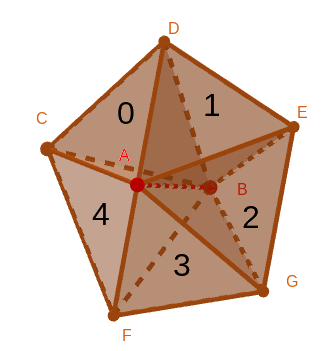
\includegraphics[scale=0.38]{Images/tetra_ordonnee}
  \caption{}
  \label{fig:tetra_ordonnee}
\end{subfigure}%
\begin{subfigure}{.5\textwidth}
  \centering
  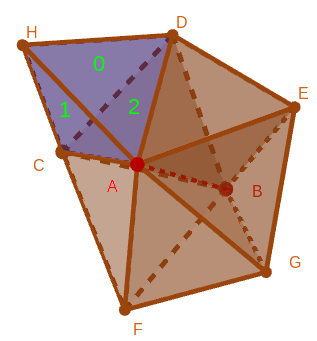
\includegraphics[scale=0.4]{Images/permutation_tetra_diamant}
  \caption{}
  \label{fig:permutation_tetra_diamant}
\end{subfigure}
\caption{\textbf{Gauche} : Diamant contenant 5 tétraèdres ordonnés, dont l'arête centrale est AB et ancré au sommet A. L'ordre des tétraèdres est indiqué en noir. L'ordre des sommets est : C,D,E,G,F,A,B. \textbf{Droite} : Un diamant partage une face avec un tétraèdre isolé. En vert est l'ordre des face du tétraèdre. L'ordre des sommets du tétraèdre est A,D,C,H et celui du diamant est C,D,E,G,F,A,B.}
\end{figure}
\subsection{Calcul des permutations}
\noindent
%Calculer les permutations des sommets entre deux faces est primordial car cela permet de connaître la position d'un sommet dans la face opposée.\\
Avec la structure naïve décrite dans la partie \ref{representation_maillages_tetra}, chaque tétraèdre possède 4 références vers ses 4 sommets. Ainsi, pour deux tétraèdres adjacents, il suffit de comparer les références de leurs sommets respectifs pour identifier les sommets communs.\\
Ici, par soucis d'économie, nous ne souhaitons pas stocker de références des tétraèdres vers leurs sommets. Nous utilisons juste l'ordre des diamants et des tétraèdres isolés afin d'identifier la position d'un sommet (partie \ref{ancrage}).\\
Néanmoins, lorsque nous passons d'une face à l'autre, nous ne savons plus associer les sommets deux à deux. Dans la Fig. \ref{fig:permutation_tetra_diamant}, cela reviendrait à ne pas savoir lors du passage du tétraèdre isolé au diamant via la face ACD où se situe le sommet A (resp. C,D). Or, deux des opérations nécessaires à notre structure de donnée sont \textbf{degree(v)} et \textbf{hypersphere(v)} qui nécessitent toutes les deux d'identifier un sommet afin de parcourir les faces adjacentes à ce sommet. Par conséquent, pour connaître l'emplacement d'un sommet dans une face opposée, nous calculons des permutations.
Dans la Fig. \ref{fig:permutation_tetra_diamant}, pour calculer la permutation vue du tétraèdre isolé de la face CAD, il suffit de comparer l'ordre des sommets du tétraèdre isolé et du diamant. Si l'on garde seulement les 3 sommets qui nous intéressent dans les deux classements, on a : A,D,C et C,D,A. La permutation est donc (2,1,0). Bien entendu, la permutation pour la même face du point de vue du diamant est la même. Il y a 3!=6 permutations possibles et donc 3 bits par face sont nécessaires pour représenter ces permutations.

\subsection{La structure}
\noindent
Désormais, nos diamants sont formés, les sommets sont associés à des diamants (ou des tétraèdres isolés) et les permutations sont calculées pour chaque face du maillage. Nous introduisons quelques notations :
\begin{itemize}
\item $D$ l'ensemble des diamants
\item $T_D$ l'ensemble des tétraèdres appartenant à des diamants
\item $T_i$ l'ensemble des tétraèdres isolés
\item $F_e$ l'ensemble des faces des tétraèdres isolés et des faces extérieures des diamants où $|F_e|=2\cdot |T_D|+4\cdot |T_i|$\\
\end{itemize}
\noindent
La structure que nous proposons est un tableau A de taille $|F_e|$. Le tableau contient des entiers représentant les indices des faces. Ainsi A[i] indique l'indice dans le tableau de la face adjacente à la ième face. Si la ième face est sur le bord du volume alors A[i]=-1.\\ 
Un diamant contenant 4 tétraèdres occupera 8 cellules dans le tableau (car il a 8 faces extérieures) et un tétraèdre isolé en occupera 4. Les diamants et tétraèdres isolés sont ré-ordonnés de tel manière que le ième sommet soit ancré au ième diamant/tétraèdre isolé. Etant donné qu'il y a beaucoup plus de diamants que de sommets, seuls, les $|V|$ premiers diamants/tétraèdres isolés sont ré-ordonnés.\\
Par ailleurs, pour savoir quand on passe d'un diamant à un autre, nous utilisons des bits de service\footnote{Un bit de service est un bit permettant de faciliter une opération. Il prend si peu de place qu'on ne le considère par comme une référence (qui est souvent codée sur 32 bits)} (1 ou 0) pour chaque face. Une face contient un 1 si c'est la première face d'un diamant/tétraèdre isolé, 0 sinon. Finalement, afin de pouvoir tourner facilement autour d'un sommet, nous utilisons 3 bits de service par face pour représenter la permutation des sommets entre ces deux faces.\\
Pour résumer, voici notre structure de données :
\begin{itemize}
\item Un tableau A de taille $|F_e|$
\item Un bit de service par face afin de savoir si une face est la première d'un diamant ou d'un tétraèdre isolé
\item 3 bits de service par face afin de représenter la permutation des sommets entre deux faces
\end{itemize}
\begin{figure}[H]
\begin{center}
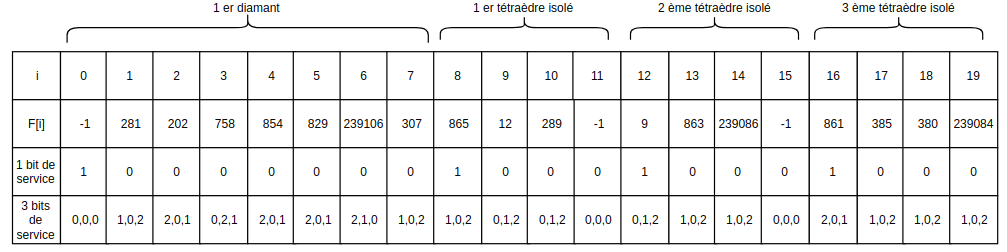
\includegraphics[scale=0.35]{Images/structure}
\caption{Notre structure est constituée d'un tableau A contenant les indices des faces adjacentes, d'un bit de service permettant de savoir si une face est la première d'un diamant ou d'un tétraèdre isolé, et de trois autres bits de service afin de connaître la permutation des sommets entre deux faces. Dans cet exemple, la face 0 est sur le bord et la face 1 est adjacente à la face 281. La permutation de la face 1 du premier diamant (1,0,2) indique que le premier et second sommets de cette face sont inversés dans la face opposée.}
\label{fig:structure}
\end{center}
\end{figure}
\subsection{Les requêtes}
\noindent
Notre structure de données permet de réaliser des requêtes simples et courantes sur le maillage. Nous détaillons dans cette partie comment ces requêtes ont été implémentées et la complexité pour chacune d'elle.
\subsubsection{Accéder à la ième face}
\noindent
Pour accéder à la ième face, il suffit d'accéder à la cellule A[i] dans laquelle se trouve la face opposée à la ième face. L'accès est donc en temps O(1).
\subsubsection{Accéder au ième diamant ou tétraèdre isolé}
\noindent
Il suffit de parcourir le tableau A et de regarder pour chaque face si le premier bit de service vaut 1. On s'arrête alors dès que l'on a parcouru i faces dont la valeur du premier bit de service est 1. En utilisant une structure adaptée au 'Rank and Select' \footnote{Dans un tableau de bits $B[0..n-1]$, $rank(x) = |\{k\in [0..x] : B[k]=1\}|$ et $select(x)=min\{k\in [0..n-1) : rank(k)=x\}$}, la compléxité est O(1) \cite{rank_and_select}.
\subsubsection{Parcourir les tétraèdres d'un diamant}
\noindent
Les faces au sein d'un diamant sont ordonnées. Les faces consécutives dans le tableau (modulo la taille du diamant) sont adjacentes dans le diamant. Par conséquent, pour accéder aux faces du jème tétraèdre d'un diamant $D_i$, il suffit d'aller aux faces d'indices $2j$ et $2j+1$ (modulo $|D_i|$). La compléxité est O(1).
\subsubsection{Accéder au ième tétraèdre}
\noindent
Lors du regroupement des tétraèdres en diamants, l'ordre des diamants n'est plus le même que l'ordre initial (à la lecture du fichier OFF). Néanmoins, on peut re-ordonner les tétraèdres dans le fichier original afin que l'ordre des tétraèdres soit les mêmes. De cette manière on peut accéder au ième tétraèdre en O(1).
\subsubsection{Accéder au ième sommet}
\noindent
Bien que nous ne stockions pas les sommets de manière explicite (nous ne stockons que les faces). Nous sommes en mesures de localiser le ième sommet car il est adjacent au ième diamant/tétraèdre isolé.
Il suffit donc d'accéder au ième diamant/tétraèdre isolé. Si c'est un diamant, alors le sommet est adjacent à toutes les faces paires du diamant. Si c'est un tétraèdre isolé, alors le sommet est opposé à la première face et est donc adjacent au trois autres faces. La complexité est la même que pour accéder au ième diamant/tétraèdre isolé, O(1).
\subsubsection{Degré et hypersphère d'un sommet}
\noindent
Calculer le degré d'un sommet est plus compliqué. On sait que le ième sommet est adjacent au ième diamant/tétraèdre isolé. Si celui-ci est un diamant alors toutes les faces paires de celui-ci sont adjacentes au sommet ciblé. Si c'est un tétraèdre isolé, alors le sommet cible est opposé à la première face et est donc adjacent aux trois autres faces. Pour chaque face adjacente au sommet on accède à la face opposée en utilisant notre tableau A. En utilisant les permutations entre deux faces, nous sommes en mesure de savoir où se situe notre sommet dans la face opposée. Ainsi, nous pouvons accéder aux faces adjacentes au sommet dans ce nouveau diamant/tétraèdre isolé. Pour chaque diamant/tétraèdre isolé, on utilise un bit de service afin de savoir si celui-ci a déjà été visité \footnote{Nous omettons ce bit de service car il y en a en moyenne $\frac{|Diamants| + |T\acute{e}tra\grave{a}dres \; isol\acute{e}s|}{|T\acute{e}tra\grave{a}dres|}\simeq 0.5$ par tétraèdre}. On arrête de parcourir les faces quand tous les diamants et tétraèdres isolés adjacents au sommet ont été visités. La complexité est donc O(d).

AJOUTER PSEUDOCODE

\subsubsection{Parcours en largeur du graphe}
\noindent
Parcourir en largeur le graphe est plus facile que de calculer le degré d'un sommet. Il suffit d'utiliser une file et un bit de service pour chaque tétraèdre afin de savoir si celui-ci a été visité. Le passage d'un tétraèdre à l'autre est rendu très facile grace à notre tableau représentant les faces adjacentes. La complexité est donc la même que dans le maillage original : O($|$T$|$).
\subsubsection{Retrouver l'indice d'un sommet}
\label{Retrouver l'indice d'un sommet}
\noindent
Retrouver l'indice d'un sommet est une procédure courante. En effet lorsque on est sur une face, on peut vouloir connaître les indices des trois sommets qui la compose. Pour connaître l'indice d'un sommet, on calcule son hypersphère. Puis pour chaque diamant ou tétraèdre isolé dans l'hypersphère dont l'indice de la première face est inférieur à la limite\footnote{La limite est l'index à partir duquel les diamant et tétraèdres isolés ne sont plus associés à des sommets}, on calcule alors l'hypersphère du sommet ancré. Il suffit de comparer l'hypersphère de notre sommet cible avec les hypersphère des sommets ancrés et de renvoyer l'indice du sommet ayant la même hypersphère. Cette opération peut s'avérer néanmoins très couteuse. La compléxité pour calculer l'hypersphère d'un sommet est O(d). En utilisant notre algorithme pour appareiller les tétraèdres en diamants, les sommets sont en moyennes adjacents à 8 diamants/tétraèdres isolés. Seulement parmi ces 8 diamants/tétraèdres isolés, en moyenne 65\% \footnote{$\frac{|Diamants|+|T\acute{e}tra\grave{e}dres\; isol\acute{e}s|}{|V|}$} auront un indice inférieur à la limite. Par conséquent, retrouver l'indice d'un sommet nécessite de calculer en moyenne 6 (0.65*8+1) hypersphères.

%\begin{tikzpicture}
%\begin{axis}[
%    title={Evolution des rpt en fonction du nombre de tétraèdres},
%    xlabel={Nombre de tétraèdres},
%    ylabel={Secondes},
%    xmin=3000, xmax=2500000,
%    ymin=0, ymax=100,
%    xmode=log,
%%    xtick={0,20,40,60,80,100},
%%    ytick={0,20,40,60,80,100,120},
%    legend pos=north west,
%    ymajorgrids=true,
%    grid style=dashed,
%]
% 
%\addplot[
%    color=blue,
%    mark=square,
%    ]
%    coordinates {
%    (3583,0.06)(83412,21.34)(125127,50.6 )(156135,96.71)(2243131,33.29)
%    };
%%    \legend{CuSO$_4\cdot$5H$_2$O}
% 
%\end{axis}
%\end{tikzpicture}

%\begin{table}[H]
%\footnotesize
%\centering
%\begin{tabular}{|c | c | c |}
%\hline
%Type de & Taille du & Mémoire consomée \\
%structure & tableau de diamant & totale (bits) \\
%\hline
%B1 & 9670 & 48374 \\
%B2 & 199314 & 996594 \\
%B3 & & \\
%M1 & 308464  & 1542344 \\
%C1 & 385248 & 1926264\\
%\hline  
%\end{tabular}
%\label{Tab:results_memory}
%\caption{Tableau décrivant la place mémoire occupée par notre structure (les 3 tableaux)}
%\end{table}
%\noindent

\subsection{Un nouveau format de stockage}
\noindent
Les fichiers OFF encodent d'abord les coordonnées géométriques de chaque sommet puis les indices des 4 sommets de chaque tétraèdre. Ils sont ainsi très faciles à manipuler mais ne sont pas concis (un sommet apparaît en moyenne 22 fois dans une tétraèdrisation). L'idée de cette section est de tirer avantage de notre appariement des tétraèdres en diamants afin de sauvegarder les maillages dans un format plus succint.
\paragraph{Encodage de la structure}
Comme exprimé dans la partie \ref{Retrouver l'indice d'un sommet}, un sommet dans notre structure est adjacent en moyenne à 8 diamants/tétraèdres isolés. Par conséquent, plutôt que de décrire pour chaque tétraèdre les 4 indices des 4 sommets, nous pouvons encoder les indices des sommets composant un diamant. Les sommets sont ordonnés dans un diamant (\ref{Ordre des sommets dans les diamants}). Ainsi, en ayant juste l'ordre des sommets, nous sommes en mesure de retrouver les faces (la première face est bordée par le premier, le deuxième et l'avant dernier sommet).\\
Cependant, notre structure ne stocke pas implicitement les sommets. Nous savons seulement que le ième sommet est adjacent au ième diamant/tétraèdre isolé. Néanmoins, en calculant l'hypersphère d'un sommet, nous informons les faces adjacentes qu'elles possèdent ce sommet. En faisant ainsi pour tous les sommets du maillage, nous associons alors à chaque face ses 3 sommets bordants.\\
Il est alors facile de retrouver l'ordre des sommets dans un diamant à partir des sommets bordants chaque face du diamant. Il suffit de prendre tous les sommets qui apparaissent exactement deux fois dans toutes les faces (i.e les sommets qui n'appartiennent pas à l'arête centrale). Puis de les ordonner afin qu'ils décrivent un cycle.\\
Par exemple, sur la Fig. \ref{fig:tetra_ordonnee}, à partir du calcul de l'hypersphère de chaque sommet, nous saurions alors que :
\begin{itemize}
\item Les faces 0 et 1 contiennent les sommets C et D
\item Les faces 2 et 3 contiennent les sommets E et D
\item Les faces 4 et 5 contiennent les sommets G et E
\item Les faces 6 et 7 contiennent les sommets F et G
\item Les faces 8 et 9 contiennent les sommets C et F\\
\end{itemize}
Trouver l'ordre des sommets est alors aisé. On commence par trouver le sommet commun à la première et dernière face (i.e C), puis le sommet commun à la première et deuxième face (i.e D) et ainsi de suite pour finalement obtenir : C,D,E,G,F,A,B (les deux derniers sommets sont communs à toute les faces).

\paragraph{Ecriture dans un fichier}
L'écriture dans un fichier suit le même procédé que pour les fichiers OFF. Nous écrivons d'abord les coordonées géométriques de chaque sommet. Puis nous écrivons pour chaque diamant et tétraèdre isolé l'ordre de ses sommmets.

\paragraph{Ouverture du fichier}
L'ouverture est similaire à l'encodage du maillage. Pour chaque diamant, l'ordre des sommets nous permet de connaître les faces. Pour chaque tétraèdre isolé, l'ordre n'est pas important étant donné que tous les sommets d'un tétraèdre sont adjacents.

\paragraph{Résultats}
En théorie comme en pratique, notre structure nous permet de reduire en moyenne la taille du fichier OFF de 44\% ($\frac{8}{18}$).

\subsection{Implémentation}
\noindent
Tout le code est implémenté en C\texttt{++} natif, sans l'aide d'aucune bibliothèque extérieure. Le code source est compilé avec g\texttt{++} sous Elementary OS. Tous les algorithmes ont été exécutés sur une machine avec un processeur i5-5300U et 16Go de RAM. L'ensemble du code est open-source et disponible sur github : \url{https://github.com/beaupletga/3D-Mesh-Compression}.\\
Des classes représentent chaque forme géométrique (sommet, tétraèdre, diamant) permettant un code modulable et facilement exploitable. Nous utilisons cette représentation sous forme de classe pour la construction de notre structure mais elle est tout à fait absente dans son utilisation. \\
En ce qui concerne cette dernière, le tableau A est un tableau d'entiers codés sur 32 bits. Bien que nous aurions pu inclure les 4 bits de services dans les 32 bits de chaque entier, nous avons préféré utiliser deux tableaux annexes pour représenter ces bits de service. Le premier bit de service est stocké dans un tableau de booléens et les 3 autres bits de service sont stockés dans un tableau d'entiers. En codant les indices dans le tableau $F$ sur 28 bits et en utilisant les 4 derniers bits comme bits de service, nous pouvons encoder des maillages ayant jusqu'à $2^{28}=268$ millions de faces.